%%% Local Variables: 
%%% mode: latex
%%% TeX-master: t
%%% End: 
\documentclass[10pt]{report}
\usepackage[utf8]{inputenc}	% UTF8 package
\usepackage{int-act}  
\usepackage{textcomp}	% common special chars
%\usepackage{amsmath}	% math formula
\usepackage{fancybox}
\usepackage{anyfontsize}	% fonts
%%\usepackage[T1]{fontenc}
\usepackage{tocloft} % formatting of the table of contents.
\usepackage{lipsum}
\usepackage{enumitem}
\usepackage{setspace}
\onehalfspacing % 1.5 line spacing
\usepackage{longtable}
\usepackage{caption}
%\usepackage[hidelinks]{hyperref}
\usepackage[raggedrightboxes]{ragged2e}
\renewcommand{\arraystretch}{1.3} 
\setlength{\extrarowheight}{2pt} 


% CHANGE %'s below to make subsection headings visible/invisible in TOC
%\newcommand{\xsubsubsection}[1]{\subsection{#1}}
\newcommand{\xsubsubsection}[1]{\subsubsection{#1}}

\def\todo#1{\textbf{TODO:} ``#1''}


\begin{document}

%%% Change log
%% format:
\istChange{01/11/2024}{v0}{EVORA}{1st Draft}

\istChange{12/11/2024}{v1.0}{EDIN}{Created template}
\istChange{30/11/2024}{v1.1}{EVORA}{Report sent to reviewer - ITML}
\istChange{2/12/2024}{v1.1}{ITML}{Revisions sent}
\istChange{9/12/2024}{v1.2}{EVORA}{Revisions incorporated}
\istChange{10/12/2024}{v1.2}{AALTO}{Revisions sent}
\istChange{12/12/2024}{v1.3}{EVORA}{Revisions incorporated}
\istChange{20/12/2024}{v1.3}{EVORA}{Report submitted}
%\istChange{24/09/2019}{v2.0}{Fábio Magalhães}{Added support for  Latin chars (áàéí etc) in changelog.}
%\istChange{25/09/2019}{submitted}{S Luz}{Redefined delivStatus to  produce $\checkmark$ for draft, final or submitted, without  affecting document identifier. Increased width
 % of version column in changelog.
 % }

%% Project and Deliverable information
%%%%%%%%%%%%%%%%%%%%%%%%%%

%% If not specified, deafults to INT-ACT
% \ProjectAcronym{INT-ACT}
%\ProjectFullTitle{Intangible Cultural Heritage, Bridging the Past, Present, and Future}
%\ProjectRefNo{101132719}
\delivNumber{D1.1}
\ContractualDate{}
\delivMonth{Novembro}
\delivYear{2024}
\delivName{Ontology Model 1}
\delivShortTile{Ontology Model 1}
%% Lead partner
\delivResponsible{EVORA} 
\delivVersion{1}
\ActualDate{December, 31 2024}
\delivDissLevel{PU - Public}
\delivType{[Report, Prototype, Other]}
\delivWP{WPx.x} % Workpackage x
\delivAuthor{Renata Vieira, António Diniz, Camila Campos, Rafael Prezado, Alicia Nunez Garcia, Áurea Rodrigues, Leonor Rocha} % autores para "EDITOR(S)"
\delivOtherContributors{%Avner Dal Bosco, 
Ivo Santos,  Saturnino Luz} % para "CONTRIBUTOR(S)"
\delivReviewer{Dora Eleftheriou, Ilektra Simitsi} % Apenas o revisor específico
\delivKeywords{[List of free keywords relevant to the deliverable]}
\delivTask{Core Concepts}
\delivTaskTitle{T1.1}
\delivTaskDuration{34 months}
\delivStatus{d} %% d = draft, f = final, s = submitted
\delivExecSummary{This deliverable consists of the Ontology Model 1 of the INT-ACT project. Along with the ontology OWL files, we deliver this report containing a brief description  of the hierarchy of concepts and instances which reflect our first case study of Cromeleque das Fontainhas in Alentejo. This first version takes into account mainly the Environment dimension. The proposed model extends the CIDOC-CRM reference model.}


\makecover


\subsection*{Disclaimer}
This document reflects the views of its author(s) and does not necessarily reflect the views or
policy of the European Commission. Whilst efforts have been made to ensure the accuracy and
completeness of this document, the European Commission is not responsible for any use that may
be made of the information it contains nor for any errors or omissions, however caused. This
document is released under Creative Commons Attribution 4.0 International License.


\newpage
\fancypagestyle{plain}{}


\settableofcontents
\tableofcontents

\newpage
\addcontentsline{toc}{section}{List of Tables} 
\setcounter{page}{5} 
\listoftables

\newpage
\addcontentsline{toc}{section}{List of Figures}
\setcounter{page}{6} 
\listoffigures

\newpage
\subsubsection*{Acronyms and abbreviations}\vspace{-1.5ex}
\addcontentsline{toc}{section}{Acronyms and Abbreviations}

\def\arraystretch{1}
\newcolumntype{a}{>{\columncolor{INT-ACTorange}}l}
  \begin{tabular}[t]{!{\color{INT-ACTorange}\vrule}a!{\color{INT-ACTorange}\vrule}l!{\color{INT-ACTorange}\vrule}}
    \arrayrulecolor{INT-ACTorange}\hline
    \color{white}
    AR &
    \color{black}
    Augmented reality
    \\\hhline{~-}
    \color{white}
    CIDOC CRM &
    \color{black}
    International Committee for Documentation Conceptual Reference Model 
    \\\hline
    \color{white}
    CDBE &
    \color{black}
    Communication, Dissemination, Exploitation, and Business Growth
    \\\hline
    \color{white}
    CF M(Number) &
    \color{black}
    Cromeleque das Fontaínhas Menhir 1-8
    \\\hline
    \color{white}
    DP &
    \color{black}
    Dissemination and Communication Plan
    \\\hhline{~-}
    \color{white}
    KPI &
    \color{black}
    Key Performance Indicator
    \\\hhline{~-}
    \color{white}
    WP &
    \color{black}
    Work Package
    \\\hhline{~-}
    \color{white}
    SIPA &
    \color{black}
    Sistema de Informação para o Património Arquitétónico
    \\\hline
   \color{white} IPA &
    \color{black}
   Inventário do Património Arquitétónico 
    \\\hline
    \color{white}
    XR &
    \color{black}
    Extended Reality 
    \\\hhline{~-}
    \color{white}
    3E &
    \color{black}
    Emotional, Experiental, and Environmental
    \\\hhline{~-}
\end{tabular}

\newpage
\section {Executive Summary} 

This deliverable describes the first ontology  model developed to represent the knowledge associated to the heritage site of the first case study.

The model was based on the CIDOC CRM model, and proposes extensions which reflect the heritage aspects relevant to the project.

The deliverable mainly consists of an owl file generated with the Protégé editor and this document explains the model rationale and describes its main concepts.

This deliverable presents the first version of INT-ACT Ontology model, which will be extended in the continuation of the project. 





















\newpage
\section{Introduction}

This report presents the initial ontology model for cultural heritage sites developed in the context of the INT-ACT project. The model is an extension of the CIDOC-CRM model\footnote{\url{https://www.cidoc-crm.org}}, in the sense that it expands the reference model by bringing in new subclasses and instances that are relevant to the project. It is relative to the case study 1,  Alentejo Megalithism, Portugal.   In particular the cultural heritage site considered for this phase of modelling is the Cromeleque das Fontainhas, which is associated to the municipality of Mora. This site was chosen due to its proximity to the Mora Museum of Megalithism, its comprehensive literature and ease of access. This version is concerned with the Environment dimension.

Whereas the project deals with the connection between \textit{Tangible} and \textit{Intangible} heritage, this first model explores in more depth the tangible aspect, by describing the heritage site 1  and establishing it as an Environment within which experiences (Experiences and Emotions - the 3Es) take place. Experiences and Emotions will be considered in more detail in the subsequent Ontology Models.

This document is organized as follows, first we mention the methods underlying the modelling work. Section 3 presents a brief characterisation of the site being modelled. A complete characterisation is given in Appendix A. Section 4 presents the new concepts proposed as an extension to CIDOC, according to the site itself, the heritage monument it holds, events and actors related to the site, its environmental surroundings. Section 5 shows the resulting hierarchy in the Protégé editor. Section 6 lists the instances associated to the defined classes having the Cromeleque das Fontainhas as the central point. Section 7 comments on the future extensions regarding properties and other related ontologies, Section 8 presents some final remarks.



\section{Method}


CIDOC CRM (Conceptual Reference Model) equips the investigator with a comprehensive formal semantic model suitable for cultural heritage data management (\cite{bruseker2017cultural}).
It enables the integration and exchanging of data from different sources to aid in the reconstruction of the past, using evidences, such has oral traditions or archaeological artefacts. In the context of the INT-ACT project, CIDOC CRM serves as a basis,  providing a framework suitable for the study of cultural heritage cases. Its  semantic definitions allow transforming localised data into a coherent global resource, facilitating in-depth analysis and ensuring consistency
\footnote{\url{https://www.cidoc-crm.org/}}.

The reference ontology's class hierarchy and property inheritance establish a hierarchical structure where broad classes like E1 CRM Entity or E2 Temporal Entity are refined into specialised sub-classes.

As the main requirement for the core concepts considered in this first model was the Environment dimension associated to Alentejo Megalithism, two CIDOC concepts were initially identified: E27 Site and E24 Physical Human Made Thing. These two concepts were expanded to further specify our case study, a megalithic site and its monuments.

CIDOC CRM also enables the correlation of different actors and events to physical or conceptual objects within specific temporal and spatial contexts.  Thus, CIDOC concepts such as E39 Actor and E5 Event are subclassified to specify the archaeologists involved in the excavation and technical analysis regarding the events occurred in the site. The Mora Museum of Megalithism is also represented as an actor, where related artefacts or explanations concerning the site are maintained and displayed. Our particular site, the Cromeleque das Fontainhas, is represented as an instance connected to the defined classes and subclasses.   

For the construction of this first model we used general well-known traditional ontology engineering methods \cite{gomez1999ontological}, considering the identification of the main concept and their relevant associated hierarchical concepts. CIDOC was used as a reference ontology from which other concepts, specifying our case study, were expanded. From the hierarchy we built description tables, which are organized according to semantic dimensions. Once the hierarchy and corresponding tables had been defined, we coded the hierarchy in the ontology editor Protegé \footnote{\url{https://protege.stanford.edu}}, producing an OWL encoded model. This is the first initial model which will be incremented in the continuation of the project. The final version will be available in the EU open research repository Zenodo \footnote{\url{https://zenodo.org}}.



\section{Cromeleque das Fontainhas: characterisation}

 The Cromeleque das Fontainhas stands out for its archaeological significance, evidenced by a circle of stones %(with dimensions and characteristics detailed in the following table) 
dating back to the Early Neolithic period and the Megalithism. With considerable cultural and historical value, the site is open to visitors and draws interest from tourists, researchers, and the general public alike. The usage of the site is still unknown and we can only assume that it would have been used for religious practices. Today it offers a unique connection to monuments from ancient civilizations. %Adicionado Early 

The described cultural heritage monument consists of a set of vertical stones, known as menhirs, intentionally positioned. This arrangement provides evidence of human occupation and activity in the past.

The Cromeleque das Fontainhas was constructed during the Early Neolithic period, specifically in the early Neolithic, approximately  7000 BC. The site was first identified in 1970, and later, in 2005 and 2006, an excavation was conducted by archaeologists Manuel Calado and Leonor Rocha. In July 17, 1990 Cromeleque das Fontainhas was classified as Property of Public Interest by decree number 29/90 by Diário da República 1st serie, Nº163, SIPA/IPA (Sistema de Informação para o Património Arquitetónico) Nº00002741. In 2011 the site has undergone through  restoration work. As of 2016 the creation of the Museum of Megalithism of Mora enabled the interpretation and preservation of the archaeological artifacts found at the site. % Adicionado informação complementar sobre a classificação do sítio e obras de restauração 

The area's climate is Mediterranean, characterized by hot, dry summers and wet winters. The landscape is rural, preserving both natural and cultural elements. The Cromeleque das Fontainhas is located in the Central Alentejo region, in the Évora district, near the town of Mora, in the locality of Pavia. The site offers a natural soundscape, filled with sounds of nature such as the rustling of tree branches, the blowing wind, and birdsong.

The archaeological artifacts uncovered at the site during the excavation are safeguarded by the Museum of Megalithism in Mora and include decorated ceramic and lithic tools from the Early Neolithic period, for example a geometric found at the site  (\cite{calado_neolitizacao_2007}). Nevertheless, the museum holds a variety of archaeological artefacts found at other megalithic sites and Neolithical settlements in the region, such as arrowheads and engraved stone slabs, known as schist plaques or plaque idols . These plaques were possibly crafted for symbolic purposes, reflecting a spiritual dimension. Additionally, the monument's menhirs feature carved engravings.


Figure \ref{fig:cat1} shows each menhir that makes up the Cromeleque das Fontainhas. Throughout this document we will  use the nomenclatures defined as "CF\_M1" as abbreviations for "Cromeleque das Fontainhas Menhir 1," and so on, as shown in the picture (\cite{calado_neolitizacao_2007}). These designations are useful for later identifying the particularities of each menhir, such as height and specific engravings, as well as associated images, drawing and photographs.

While the site itself represents the tangible heritage, for the intangible heritage, the project will consider a group  of narratives, with stories conveying valuable memories and add meaning to the site.  Audio files may represent the local soundscape, presenting the site´s unique acoustic environment. The cromlechs are documented through images and videos, also 3D, providing a visual representation of the monuments and strengthening the connection between the past, present and future.

\begin{figure}[!ht]
\centering
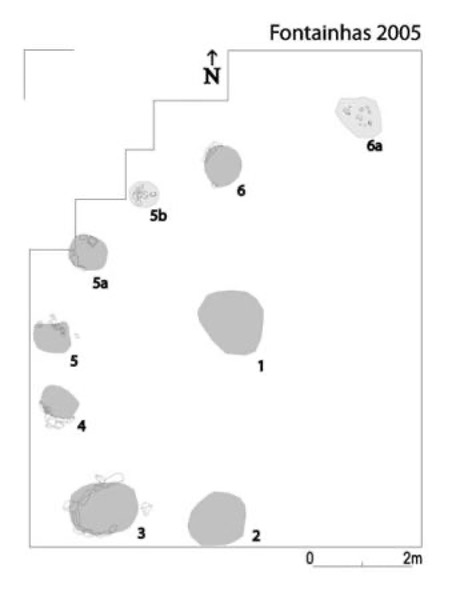
\includegraphics[width=0.4\linewidth]{figures/horseshoeimg.jpg}
\caption{\label{fig:cat1}Cromeleque das Fontainhas (\cite{calado_neolitizacao_2007}).}
\end{figure}




\section{CIDOC extensions: new concepts}\label{sec-newconcepts}

In this section we present the concepts included in our extension of CIDOC concepts, according to the brief overview given in the last session. Here the ideas are organized following a logic based structure, typical of ontologies. We divided these concepts into several dimensions, as follows.



\begin{itemize}
    \item Concepts specifying the site itself, table \ref{tab-site};
    \item Concepts specifying the monument, table \ref{tab-monument};

    \item Events and actors, table \ref{tab-eventactors};
    \item The environmental surroundings, table \ref{tab-env};

    \item Complementary components of the monument, table \ref{tab-components};
         
    \item Intangible elements, table \ref{tab-int}.
\end{itemize}

The tables present the name of the concept, its description, and its superclass. All CIDOC concepts are identified by its index number.

\begin{longtable}{|p{1in}|p{2.5in}|p{2.5in}|}
    \caption{\textbf{Site Dimension}: Concepts related to the heritage site typology}
    \label{tab-site} \\
    \hline
    Name & Description & Superclass \\
    \hline \hline 
    Archaeological Site & The area where traces of human occupation have been found & E27 Site \\
    \hline 
    Megalithic Site & A specific geographical area where large stone monuments or constructions, like stones circles or standing stones, are located & Archaeological Site \\
    \hline 
    Touristic Site & A space open to visitors & E27 Site \\
    \hline 
    Cultural Heritage Site & A place of importance recognised for its historical and cultural value & E27 Site \\
    \hline 
    Spiritual Ritual Site & A location where ancient religious or ceremonial/ritualistic practices were/are conducted & E27 Site \\
    \hline
\end{longtable}

\begin{longtable}{|p{1in}|p{2.5in}|p{2.5in}|}
    \caption{\textbf{Monument Dimension}: Concepts related to the heritage monument typology and components}
    \label{tab-monument} \\
    \hline
    Name & Description & Superclass \\
    \hline \hline 
    Cultural Heritage Monument & A Heritage monument related to a nation or a group of people & E24 Physical Human Made Thing \\
    \hline 
    Archaeological Monument & A monument that preserves traces of human occupation & Cultural Heritage Monument \\
    \hline 
    Megalithic Monument & An archaeological monument built with standing megalithic stones & Archaeological Monument \\
    \hline 
    StoneCircle\slash Cromlech & An arrangement of standing stones (menhirs) placed by humans  & Megalithic Monument \\
    \hline
    Menhir & A standing stone placed in the ground by humans & Megalithic Monument \\
    \hline
\end{longtable}




\begin{longtable}{|p{1in}|p{2.5in}|p{2.5in}|}
    \caption{\textbf{Events Dimension}: Concepts related to events, actors and time associated with the monument}
    \label{tab-eventactors} \\
    \hline
    Name & Description & Superclass \\
    \hline \hline 
    \endfirsthead
    
    \multicolumn{3}{c}%
{{\bfseries Table \thetable\ Continued from previous page (Events Dimension)}} \\
\hline
   Name & Description & Superclass \\
    \hline \hline 
\endhead    
    Neolithic & A specific period from the pre-history & E4 Period \\
    \hline
    Early Neolithic & The earliest phase of the Neolithic & Neolithic \\
    \hline
    Excavation & Technical examination of an archaeological site which involves the digging and removal of layers of earth and their associated artefacts & E5 Event \\
    \hline 
    Identification & The identification of the archaeological site & E5 Event \\
    \hline 
    Construction & The construction of the archaeological site & E5 Event \\
    \hline
    Occupation/ Usage & The occupation or usage of the archaeological site & E5 Event \\
    \hline 
    Recovery & The recovery of components of the archaeological site & E5 Event \\ %Adicionado a Classe Recovery
    \hline
    TimeSpan & The interval of time between two points during which an event occurs & E52 TimeSpan \\
    \hline
    Archaeologist & A professional whose expertise involves both on-site and off-site study of past human societies & E39 Actor \\
    \hline 
    Museum & A public space whose efforts involve the acquisition, preservation, research and exhibition of objects with different types of values & E39 Actor \\
    \hline 
\end{longtable}

\begin{longtable}{|p{1in}|p{2.5in}|p{2.5in}|}
    \caption{\textbf{Environment Dimension}: Concepts related to the environmental surroundings}
    \label{tab-env} \\
    \hline
    Name & Description & Superclass \\
    \hline \hline     \endfirsthead
    
    \multicolumn{3}{c}%
{{\bfseries Table \thetable\ Continued from previous page (Environment Dimension)}} \\
\hline
   Name & Description & Superclass \\
    \hline \hline 
\endhead    
    Climate & A feature regarding weather conditions & E26 Physical Feature  \\
    \hline
    Landscape & Landscape includes physical and natural elements, as well as human elements such as built structures & E26 Physical Feature \\
    \hline
    Cultural Landscape & A landscape containing features made by humans. It can be protected has a cultural heritage site & Landscape \\
    \hline
    Rural Landscape & A field characterized by green areas with diverse vegetation & Cultural Landscape \\
    \hline
    Urban Landscape & This type of landscape refers to a space like a city that contains physical and visual elements built by humans & Cultural Landscape \\
    \hline
    Soundscape & Set of sounds typical from an environment & E26 Physical Feature \\
    \hline
    Natural Soundscape & Sounds of nature in its characteristic environment & Soundscape \\
    \hline
    Bird sounds & The sounds of birds chirping & Natural soundscape \\
    \hline
    Tree Branches sounds & The sounds of tree Branches moving & Natural soundscape \\
    \hline
    Wind blowing sounds & The sounds of the wind blowing & Natural soundscape \\
    \hline
    Region & A geographical unit that can aggregate multiple districts & E53 Place \\
    \hline
    District & A subdivision of a region that can encompass multiple municipalities within boundaries & E53 Place \\
    \hline
    Municipality & The second-level administrative division after the district, with its own jurisdiction and local government & E53 Place \\
    \hline
    Parish & A minor administrative division, sub part of Municipalities & E53 Place \\
    \hline
    Coordinates & A specific location in space & E94 Space Primitive \\
    \hline
\end{longtable}

\begin{longtable}{|p{1in}|p{2.5in}|p{2.5in}|}
    \caption{\textbf{Artefacts Dimension}: Concepts related to complementary components of the heritage monument}
    \label{tab-components} \\
    \hline
    Name & Description & Superclass \\
    \hline \hline 
    Archaeological Artefact & Artefacts found in an archaeological site & E24 Physical Human Made Thing \\
    \hline
    Arrowhead & The tip of an arrow & Archaeological Artefact \\
    \hline
    Loom weight & Object used in textile production & Archaeological Artefact \\
    \hline
    Idol & Made with the purpose of fulfilling a religious / ritualistic / symbolic goal & Archaeological Artefact \\
    \hline
    Plaque Idol & An idol with the shape of a plaque (engraved stone plaques) & Idol \\
    \hline
    Engravings & Engravings/ Decorations on the menhirs & E90 Symbolic Object \\
    \hline
\end{longtable}

\begin{longtable}{|p{1in}|p{2.5in}|p{2.5in}|}
    \caption{\textbf{Intangible Dimension}: the intangible elements concerning the heritage site}
    \label{tab-int} \\
    \hline
    Name & Description & Superclass \\
      \hline \hline
    \endfirsthead
   
    \multicolumn{3}{c}%
{{\bfseries Table \thetable\ Continued from previous page (Intangible Dimension)}} \\

\hline 
    Name & Description & Superclass \\

 \hline \hline   
 \endhead  
    Audio & Audio files & E31 Document \\
    \hline    
    Images & Image files & E31 Document \\
    \hline    
    Narratives & A story that transmits meaning and significant memories of a specific place & E33 Linguistic Object \\
    \hline  
\end{longtable}





\section{Class hierarchy in Protégé}

The concepts described above compose the ontology hierarchy, which was edited in Protegé\footnote{\url{https://protege.stanford.edu}}. Figures \ref{fig:cat1a} and \ref{fig:cat1b} show the hierarchy of concepts, respecting CIDOC´s original hierarchy (version 7.3). CIDOC identifier labels were maintained,  thus, all CIDOC concepts starts with \textit{E(number)\_}, while all others are our proposed extensions. The resulting model, handed in this deliverable, is an owl version of the proposed extensions, which also includes CIDOC previously defined concepts. 

\begin{figure}[!ht]
\centering
\begin{minipage}{0.5\textwidth}
    \centering

    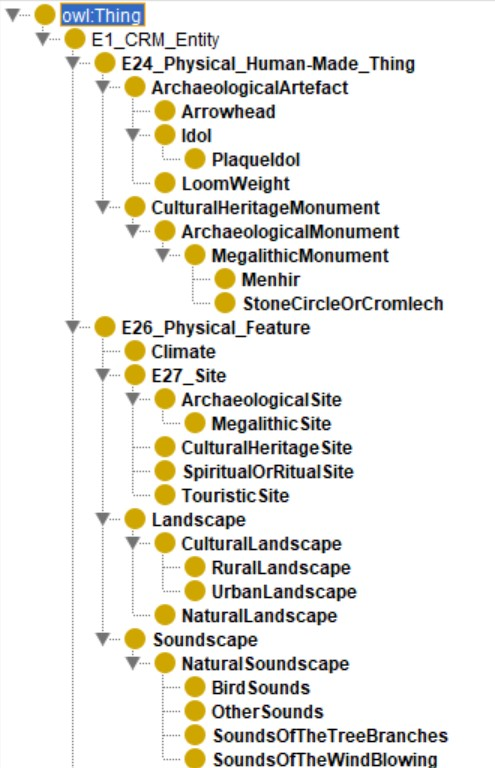
\includegraphics[height=0.5\textheight]{figures/OntoAlinhada_Atualizada.jpg}
    \caption{\label{fig:cat1a}Class hierarchy (a).}
    
\end{minipage}\hfill
\begin{minipage}{0.5\textwidth}
    \centering
    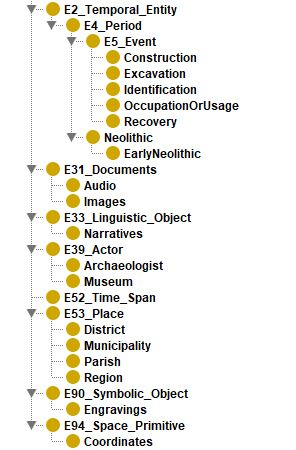
\includegraphics[height=0.5\textheight]{figures/Onto_Alinhada2.JPG}
    \caption{\label{fig:cat1b}Class hierarchy (b).}
    
\end{minipage}
\end{figure}

%\caption{\label{fig:cat1}Cromeleque das Fontainhas.}




\section{Instances}\label{sec-instances}

After the concepts, we indicate the individuals (instances) that are under analysis in the INT-ACT project. In this version, we are modelling Cromeleque das Fontainhas. The instance tables present the  name of the represented instance, its description, and the associated classes (from those defined in the previous tables 1 to 6), as follows. 

\begin{itemize}
    \item Instances regarding  the site itself, and its monument, table \ref{tab-inst-site};
   
    \item Instances regarding events and actors, table \ref{tab-inst-eventactors};
    
    \item Instances regarding the environmental surroundings, table \ref{tab-inst-env} ;  

 \item Instances regarding the concepts specifying the monument complements, table \ref{tab-inst-mon}.
 
\end{itemize}


The instances are also codified in the model, Figure \ref{fontainhas-inst} shows a Protégé instance view of Cromeleque das Fontainhas based on the model. The example of Figure \ref{menir-inst} refers to menhir CF\_M1. Whereas tables show only the closest superclass, the figures of Protégé instance view show the complete hierarchy of the instances.


\begin{longtable}{|p{1.5in}|p{2in}|p{2in}|}
    \caption{Instances related to the site regarding the concepts of Table 1/2}
    \label{tab-inst-site} \\
    \hline
    Name & Description & Class \\
    \hline \hline
    Cromeleque das Fontainhas & A stone circle located between Mora-Pavia in Portugal & -StoneCircle/Cromlech \newline - Megalithic Site \newline -Touristic Site \newline -Cultural Heritage Site \\
    \hline
    CF\_M1, CF\_M2, CF\_M3, CF\_M4, CF\_M5, CF\_M5a, CF\_M5b, CF\_M6, CF\_M6a, CF\_M7, CF\_M8 & Individual megalithic monument/monuments of the Cromeleque das Fontainhas & Menhir \\ %Adicionado CF_M7 e CF_M8
    \hline
\end{longtable}



\begin{figure}[!ht]
\centering
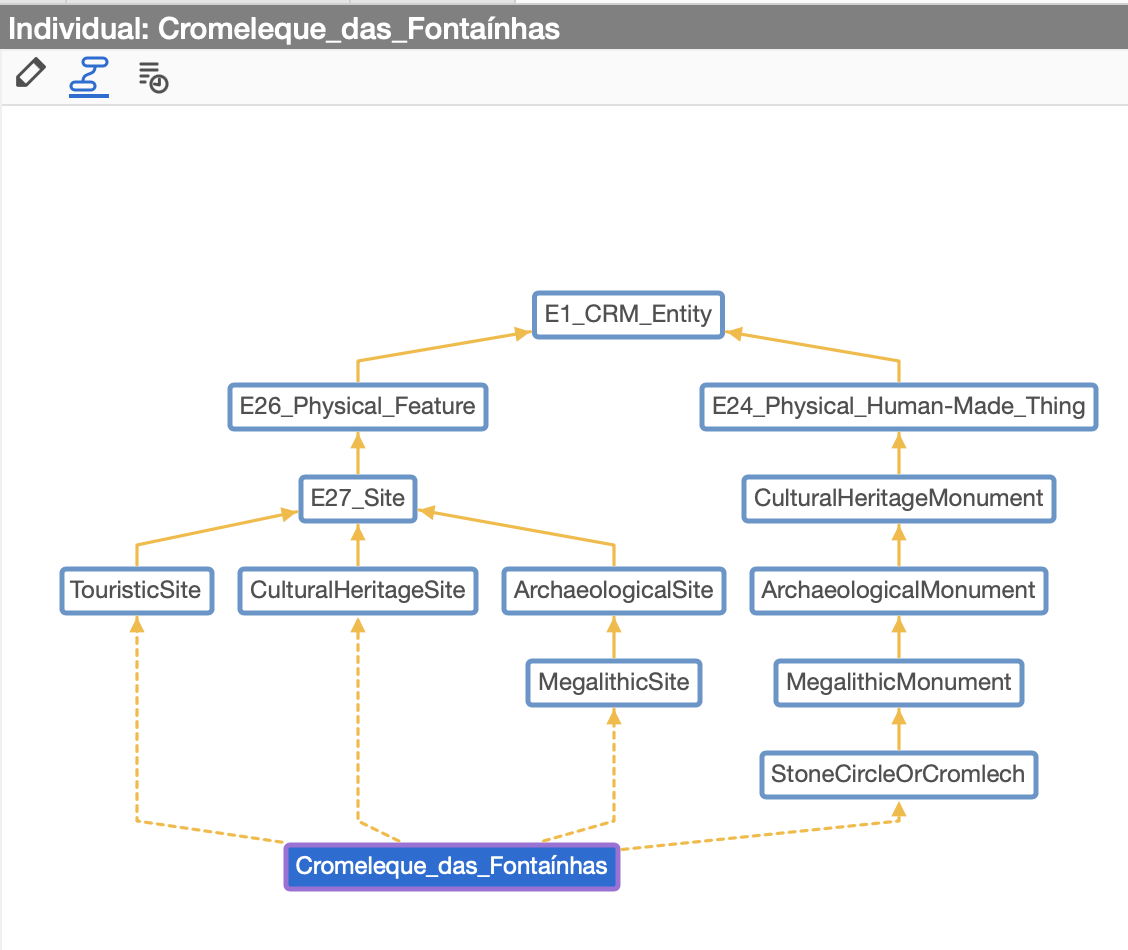
\includegraphics[width=0.8\linewidth]{figures/fontainhas-instance.png}
\caption{\label{fontainhas-inst} Protégé instance view: Cromeleque das Fontainhas}
\end{figure}

\begin{figure}[!ht]
\centering
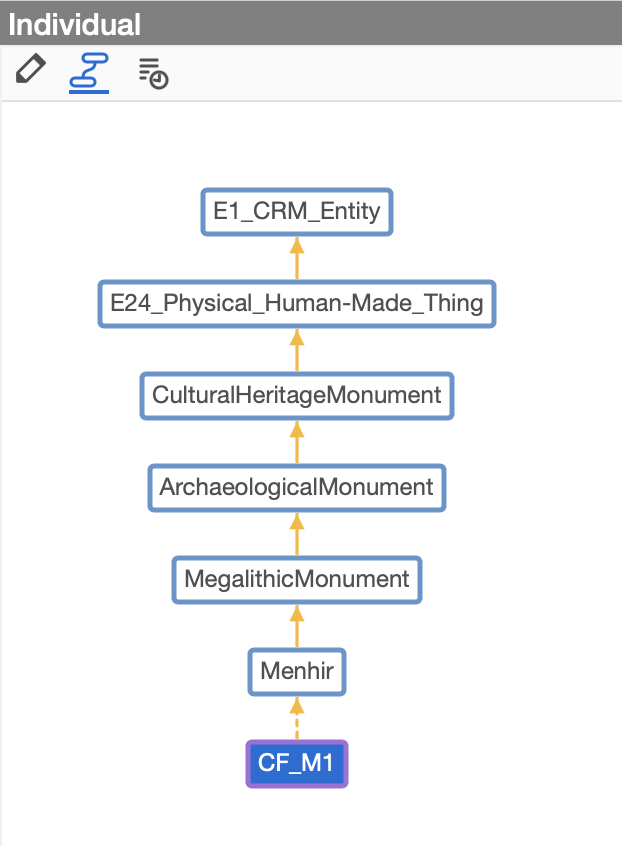
\includegraphics[width=0.5\linewidth]{figures/menir-inst.png}
\caption{\label{menir-inst} Protégé instance view: Menhir CF\_M1}
\end{figure}


\begin{longtable}{|p{1.5in}|p{3in}|p{1in}|}
    \caption{Instances related to the Events and Actors of Table \ref{tab-eventactors}}
    \label{tab-inst-eventactors} \\
    \hline
    Name & Description & Class \\
    \hline \hline
    \endfirsthead
    
    \multicolumn{3}{c}%
{{\bfseries Table \thetable\ Continued from previous page (Instances of Events and Actors)}} \\
\hline
   Name & Description & Class \\
    \hline \hline 
\endhead    
    
    \~7000-2000\~ & The time between the years \~7000-2000\~ & E52 Time Span \\
    \hline
    2005-2006 & The time between the years 2005-2006 & E52 Time Span \\
    \hline
    1970 & The year of 1970 & E52 Time Span \\
    \hline
    Manuel Calado & An Archaeologist specialized in Alentejo Megalithism & Archaeologist \\
    \hline
    Leonor Rocha & An Archaeologist specialized in Alentejo Megalithism & Archaeologist \\
    \hline
     Pedro Alvim & An Archaeologist specialized in Alentejo Megalithism & Archaeologist \\ %Adicionado Pedro Alvim 
    \hline
    Museu do Megalitismo de Mora & The Megalithic Museum located in Mora & Museum \\
    \hline
    Excavation of Cromeleque das Fontainhas & The event of archaeological excavation of Fontainhas & Excavation \\
    \hline
    Identification of Cromeleque das Fontainhas & The event of archaeological identification of Fontainhas & Identification \\
    \hline
    Occupation or Usage of Cromelque das Fontainhas & The event of occupation of the site, according to the archaeological findings & Occupation/ Usage \\
    \hline
    Construction of Cromeleque das Fontainhas & The event of constructing the site & Construction \\
    \hline
    Recovery of Cromeleque das Fontainhas & The event of recovering the site & Recovery \\ %Adicionado Recovery 
    \hline
\end{longtable}

\begin{longtable}{|p{1.5in}|p{3in}|p{1in}|}
    \caption{Instances related to the environment surroundings regarding the concepts of Table \ref{tab-env}}
    \label{tab-inst-env} \\
    \hline
    Name & Description & Class \\
    \hline \hline
    Alentejo Central & A region of Portugal & Region \\
    \hline
    District of Évora & A district of Portugal & District \\
    \hline
    Mora & A municipality in the district of Évora & Municipality \\
    \hline
    Pavia & A parish in the municipality of Évora & Parish \\
    \hline
    38.931079, -8.121081 & GPS coordinates & Coordinates \\
    \hline
    Mediterranean Climate & The climate of the Mediterranean region & Climate \\
    \hline
    Montado Alentejano & A landscape in Alentejo/Portugal & Landscape \\
    \hline
\end{longtable}


\begin{longtable}{|p{1.5in}|p{3in}|p{1in}|}
    \caption{Instances related to the components of the monument as in Table \ref{tab-components}}
    \label{tab-inst-mon} \\
    \hline
    Name & Description & Class \\\hline \hline
%    Horseshoe shape & A specific formation where the standing stones are arranged in a U-shaped layout & Format 
%\\
%\hline
       Sandstone Plaque from Coudelaria de Alter & A plaque made of sandstone found in Coudelaria de Alter & Plaque Idol \\
    \hline
    Crescent and Crozier & A type of symbolic decoration from pre-history & Decoration \\
    \hline
    \end{longtable}






\newpage

\section{Future extensions}

\subsection{Properties}

The first version contains only the hierarchy of core concepts. Properties are not yet codified, however, the study of relevant properties has started. Data properties and object properties will define attributes and relations among the classes. For a better understanding of how the classes will be connected in the future versions, examples of properties are given in Tables \ref{tab-dataprop} and \ref{tab-objprop} respectively. We will consider CIDOC properties already defined whenever possible, they are identified in the examples with their original \textit{P(number)} id.



\begin{longtable}{|p{1.6in}|p{2in}|p{1.5in}|}
    \caption{Examples of data property definitions} \label{tab-dataprop} \\ 
    \hline
    \textbf{Class (Domain)} & \textbf{(Data property)} & \textbf{Value (Range)} \\
    \hline
    \endfirsthead
     \multicolumn{3}{c}%
{{\bfseries Table \thetable\ Continued from previous page (Examples of Data Property)}} \\
    \hline
    \textbf{Class (Domain)} & \textbf{(Data property)} & \textbf{Value (Range)} \\
    \hline
    \endhead
    \hline
    \endfoot
    \hline
    \endlastfoot
    E27 Site & usageTypeMegalithism & (string) Funerary, Non Funerary \\
    \hline
    Megalithic Monument & rockType & (string) Granite, Unknown \\
    \hline
    Megalithic Monument & format & (string) Horse shoe shape, Circular shape \\
    \hline
    Menhir & heightMeters & (decimal) \\
    \hline
\end{longtable}

\begin{longtable}{|p{1.6in}|p{2in}|p{1.5in}|}
    \caption{Examples of object property definitions} \label{tab-objprop} \\
    \hline
    \textbf{Class (Domain)} & \textbf{Relation (Property)} & \textbf{Class (Range)} \\
    \hline
    \endfirsthead
    \hline
    \textbf{Class (Domain)} & \textbf{Relation (Property)} & \textbf{Class (Range)} \\
    \hline
    \endhead
    \hline
    \endfoot
    \hline
    \endlastfoot
    Temporal Entity (Event) & P4 hasTimeSpan & E52 TimeSpan \\
    \hline
    E4 Period (Event) & P8 took place on or within & E18 Physical Thing (Archaeological Site) \\
    \hline
    E18 Physical Thing (Megalithic Monument) & P46 is composedOf & E18 Physical Thing (Menhir) \\
    \hline
\end{longtable}





\subsection{Other reference ontologies}

While the current version of the model refers to CIDOC, future associations to domain ontologies are in the work plan. One of such related ontologies is the  Environment Ontology, 
Envo \footnote{\url{https://sites.google.com/site/environmentontology/Browse-EnvO?authuser=0}, \\ \url{http://purl.obolibrary.org/obo/ENVO_01001200}
}{(\cite{buttigieg2013environment})}. This ontology brings specialized concepts regarding the environment, such as the 
concept: anthropised terrestrial environmental zone, 
defined as: 
\textit{A terrestrial zone which is bounded by constructed, manufactured, or other anthropogenic material entities.}

The hierarchy (see below) leads to different classes of rural area or areas of developed space with high usage intensity, which might help characterize the project's different sites.

\begin{verbatim}
+ entity
+ continuant
+ independent continuant
+ material entity
+ fiat object
+ environmental zone
+ terrestrial environmental zone
+ anthropised terrestrial environmental zone
- rural area
- area of developed open space
- area of pastureland or hayfields
- area of developed space
- area of developed space with low usage intensity
- area of developed space with medium usage intensity
- area of developed space with high usage intensity
- business park    
\end{verbatim}



Another example is 
ICON: An Ontology for Comprehensive Artistic Interpretations\footnote{\url{https://dl.acm.org/doi/full/10.1145/3594724
}} (\cite{sartini2023icon}),  an ontology that models artistic interpretations of artworks’ subject matter (i.e., iconographies) and meanings (i.e., symbols, iconological aspects). 
The ontology exploits symbolic interpretations, intrinsic meanings, and the motifs through which their subjects are represented. One of their research questions is: 	
To what extent is it possible to model the domain of knowledge of iconology and iconography, to provide art historians and cultural institutions a way for expressing complex art subjects and meanings, the interlinking among them, and claims about their interpretations?

We believe these ideas may serve as good insight for dealing with questions related to heritage interpretation.


%\newpage




%--- Section ---%
\section{Final remarks}

This report explains the first ontology model developed in the context of the INT-ACT project, based on CIDOC-CRM. The heritage site and its environment is characterized through a hierarchy of classes, highlighting relevant dimensions of the heritage site according to case study 1, Megalithism in Alentejo. 

For the future, the ontology model will be complemented with the class properties. The properties will further define the  connections between concepts and specific characteristics. Then instances for case study 2, related to the Calanais megalithic monuments,  will be added. The other sites (Koli and Kavála) will also be analysed and new classes will be considered.






\clearpage
\phantomsection
\addcontentsline{toc}{section}{Bibliography}
\renewcommand{\bibname}{Bibliography}
\vspace*{-2.5cm}
\section*{\bibname}
\vspace*{1cm}
\printbibliography[heading=none]





%\newpage
%\section{Appendix}


\end{document}
